\documentclass{sigchi}

% Use this command to override the default ACM copyright statement (e.g. for preprints). 
% Consult the conference website for the camera-ready copyright statement.


%% EXAMPLE BEGIN -- HOW TO OVERRIDE THE DEFAULT COPYRIGHT STRIP -- (July 22, 2013 - Paul Baumann)
% \toappear{Permission to make digital or hard copies of all or part of this work for personal or classroom use is 	granted without fee provided that copies are not made or distributed for profit or commercial advantage and that copies bear this notice and the full citation on the first page. Copyrights for components of this work owned by others than ACM must be honored. Abstracting with credit is permitted. To copy otherwise, or republish, to post on servers or to redistribute to lists, requires prior specific permission and/or a fee. Request permissions from permissions@acm.org. \\
% {\emph{CHI'14}}, April 26--May 1, 2014, Toronto, Canada. \\
% Copyright \copyright~2014 ACM ISBN/14/04...\$15.00. \\
% DOI string from ACM form confirmation}
%% EXAMPLE END -- HOW TO OVERRIDE THE DEFAULT COPYRIGHT STRIP -- (July 22, 2013 - Paul Baumann)


% Arabic page numbers for submission. 
% Remove this line to eliminate page numbers for the camera ready copy
% \pagenumbering{arabic}


% Load basic packages
\usepackage{balance}  % to better equalize the last page
\usepackage{graphics} % for EPS, load graphicx instead
\usepackage{times}    % comment if you want LaTeX's default font
\usepackage{url}      % llt: nicely formatted URLs

% llt: Define a global style for URLs, rather that the default one
\makeatletter
\def\url@leostyle{%
  \@ifundefined{selectfont}{\def\UrlFont{\sf}}{\def\UrlFont{\small\bf\ttfamily}}}
\makeatother
\urlstyle{leo}


% To make various LaTeX processors do the right thing with page size.
\def\pprw{8.5in}
\def\pprh{11in}
\special{papersize=\pprw,\pprh}
\setlength{\paperwidth}{\pprw}
\setlength{\paperheight}{\pprh}
\setlength{\pdfpagewidth}{\pprw}
\setlength{\pdfpageheight}{\pprh}

% Make sure hyperref comes last of your loaded packages, 
% to give it a fighting chance of not being over-written, 
% since its job is to redefine many LaTeX commands.
\usepackage[pdftex]{hyperref}
\hypersetup{
pdftitle={SIGCHI Conference Proceedings Format},
pdfauthor={LaTeX},
pdfkeywords={SIGCHI, proceedings, archival format},
bookmarksnumbered,
pdfstartview={FitH},
colorlinks,
citecolor=black,
filecolor=black,
linkcolor=black,
urlcolor=black,
breaklinks=true,
}

% create a shortcut to typeset table headings
\newcommand\tabhead[1]{\small\textbf{#1}}


% End of preamble. Here it comes the document.
\begin{document}

\title{Comparing Traditional and Touch Environments for Medical Image Diagnosis}

\numberofauthors{3}
\author{
  \alignauthor Francisco Maria Calisto\\
    \affaddr{Affiliation}\\
    \affaddr{Address}\\
    \email{francisco.calisto@tecnico.ulisboa.pt}\\
    \affaddr{Optional phone number}
  \alignauthor 2nd Author Name\\
    \affaddr{Affiliation}\\
    \affaddr{Address}\\
    \email{e-mail address}\\
    \affaddr{Optional phone number}    
  \alignauthor 3rd Author Name\\
    \affaddr{Affiliation}\\
    \affaddr{Address}\\
    \email{e-mail address}\\
    \affaddr{Optional phone number}
}

\maketitle

\begin{figure}[h]
\centering
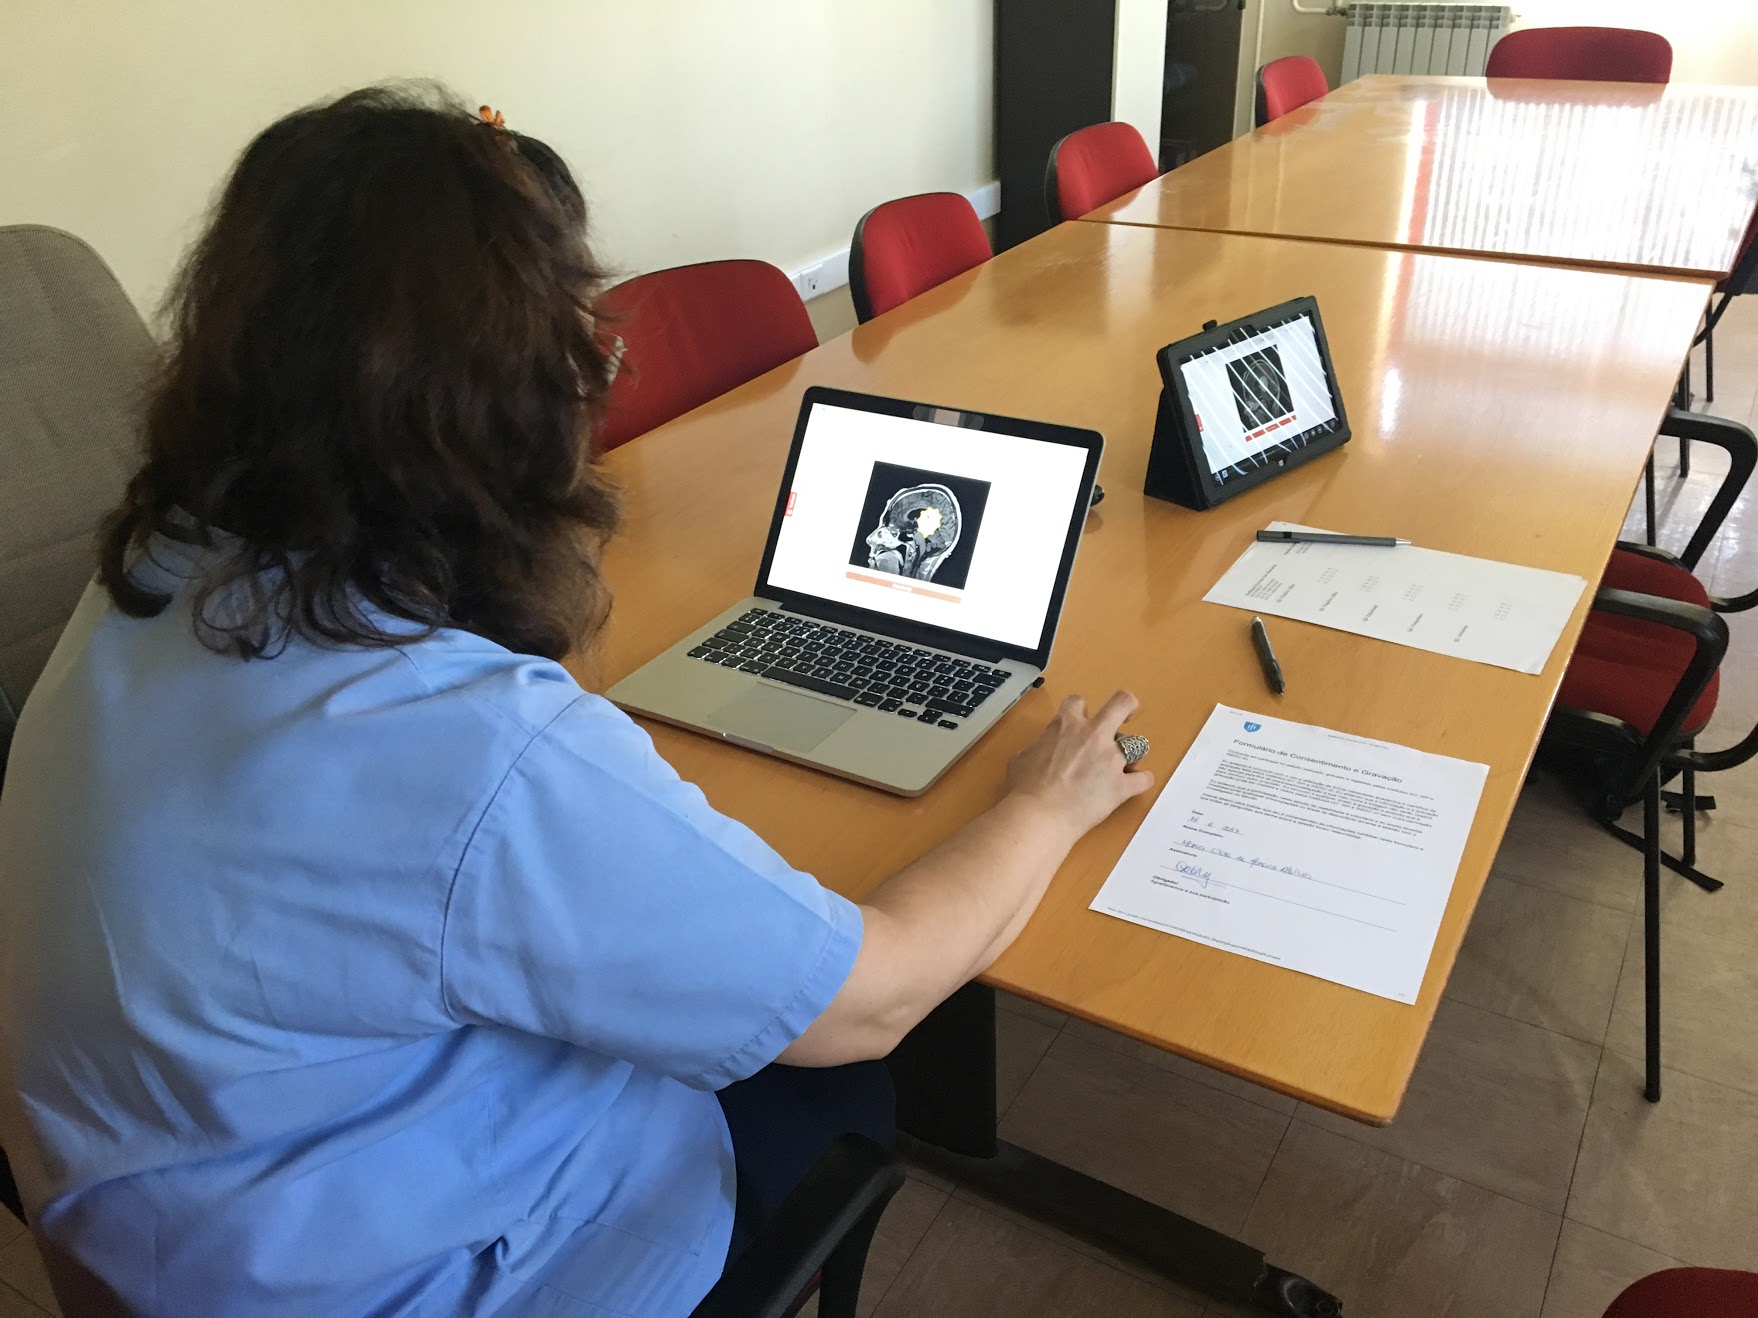
\includegraphics[width=1.0\columnwidth]{IMG_4987.JPG}
\caption{Physician Radiologist interacting with traditional environment.}
\label{fig:Fig1}
\end{figure}

\begin{figure}[h]
\centering
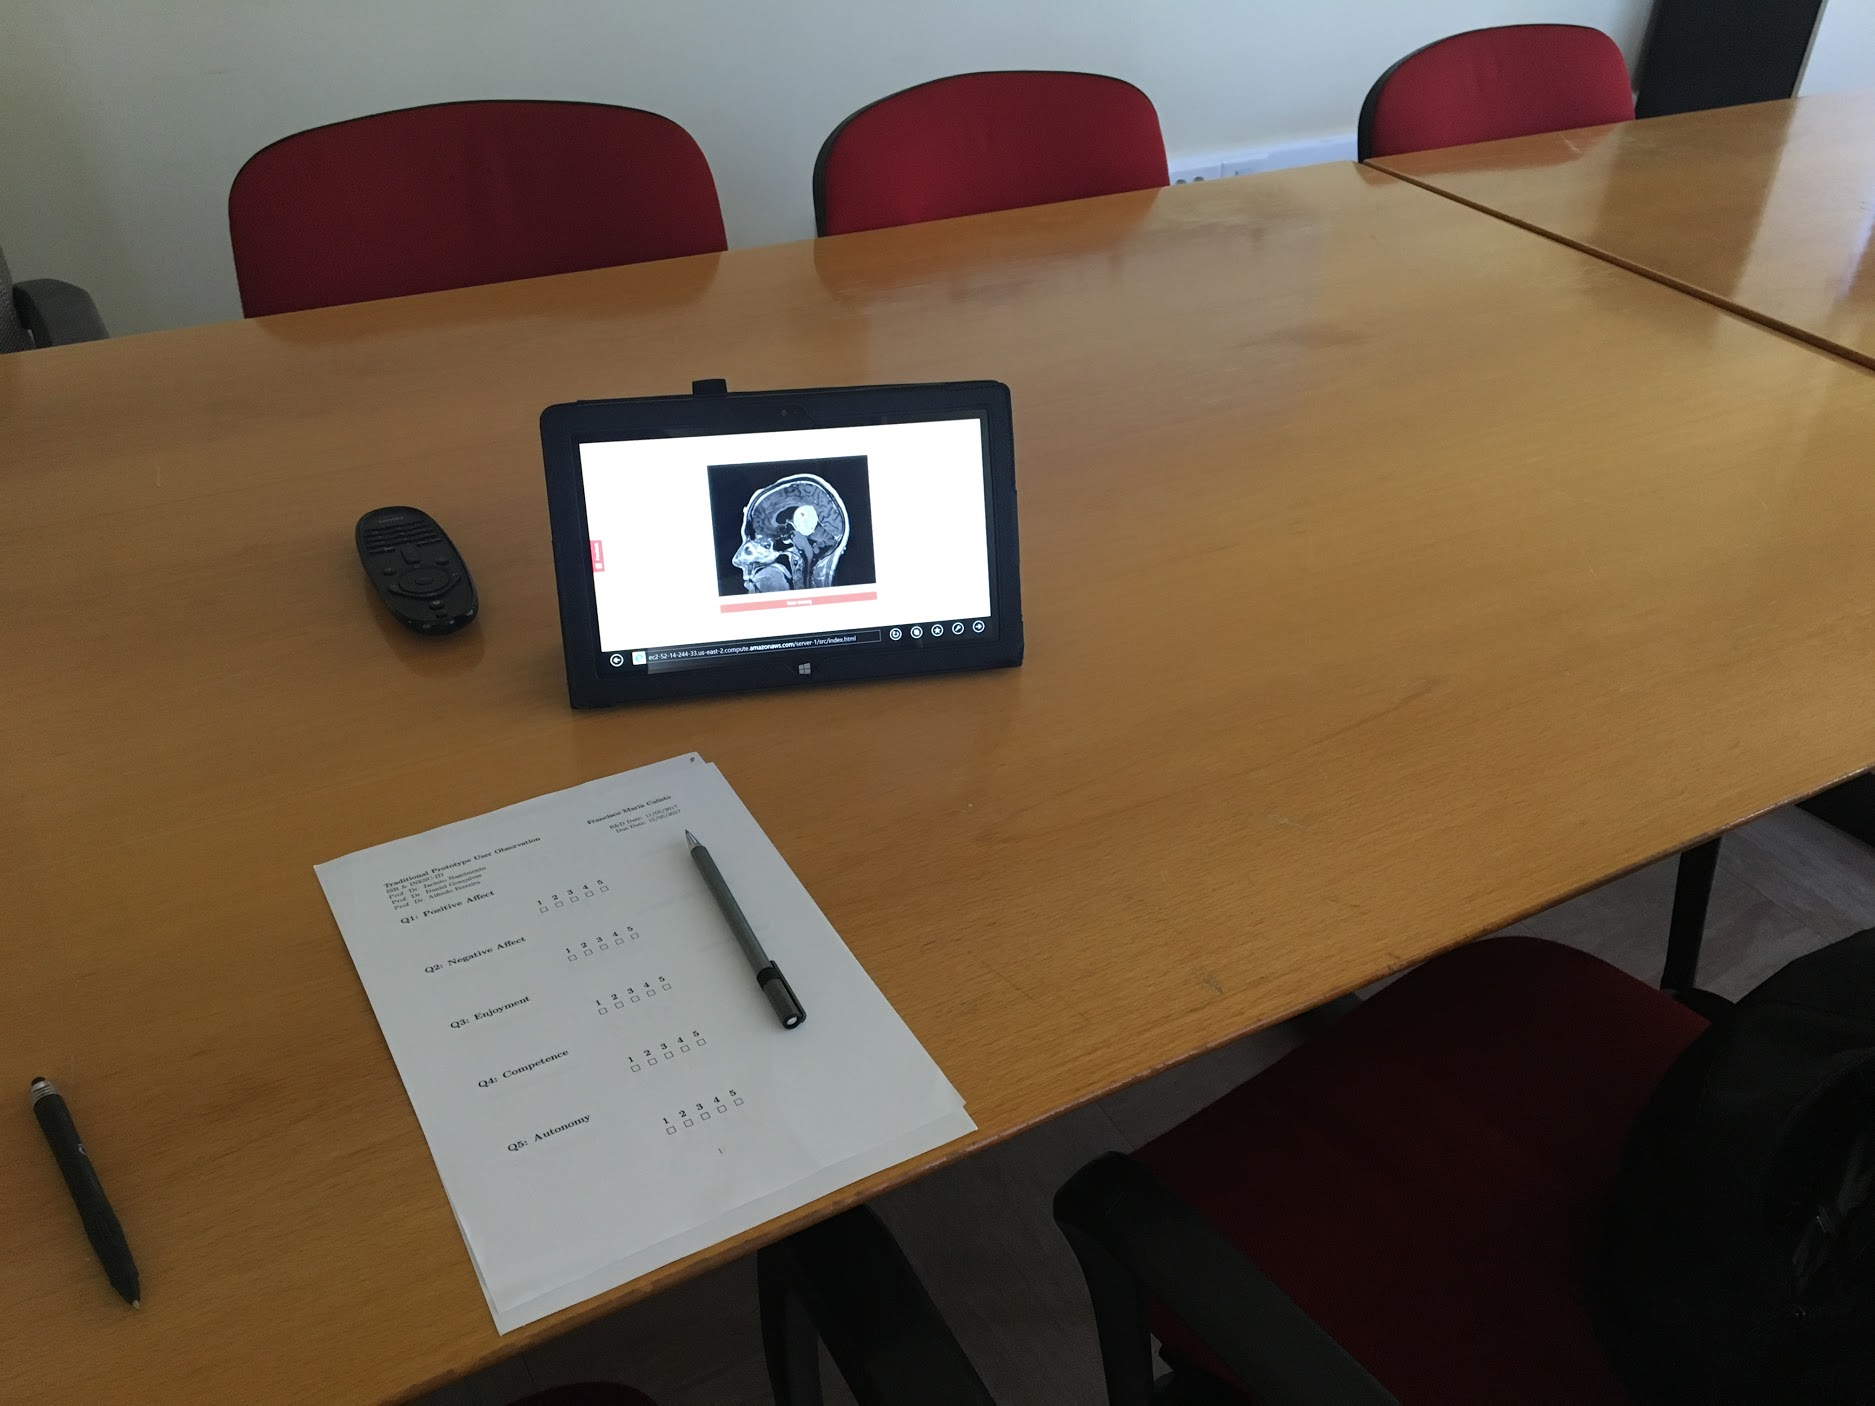
\includegraphics[width=1.0\columnwidth]{IMG_4979.JPG}
\caption{User Testing room with touch environment.}
\label{fig:Fig2}
\end{figure}

\begin{abstract}

It is becoming increasingly apparent in medical image analysis that multiple imaging modalities are required for the accurate treatment and diagnosis of the disease. Our work is to  evaluate the performance and differences between direct touch and traditional (keyboard and mouse) input on two different devices using several validated scales. The proposed problem will help a research data collection, since it will help us understand the right environment to collect those data artifacts for a clinical purpose.

\end{abstract}

\keywords{
	Guides; instructions; author's kit; conference publications;
	keywords should be separated by a semi-colon. \newline
	\textcolor{red}{Optional section to be included in your final version, 
  but strongly encouraged.}
}

\category{H.5.m.}{Information Interfaces and Presentation (e.g. HCI)}{Miscellaneous}

See: \url{http://www.acm.org/about/class/1998/}
for more information and the full list of ACM classifiers
and descriptors. \newline
\textcolor{red}{Optional section to be included in your final version, 
but strongly encouraged. On the submission page only the classifiers’ 
letter-number combination will need to be entered.}

\section{Introduction}

The medical imaging diagnosis is a topic of great interest, it has been the subject of intensive research in the world of medicine, and more specifically to Radiology. However the developments in terms of innovation in the computational world are still scarce. The user interfaces herein proposed deals with the analysis of digital images, commonly used by medical community. Related to the ease of distribution, retrieval and storage reasons, where digital images have a positive impact on medical diagnosis.

In the proposed paper, i.e., an analysis of the performance and differences between direct touch and traditional environments, several issues must be considered. First, each environment must be comfortable to interact with and fast enough, to solve the annotation improvements. Second, for each environment, a simple image feature must be considered.

\clearpage

The performance differences of traditional and touch input have been studied in terms of speed and accuracy for clinical and medical variety of interactive tasks, such as Regions of Interest (ROI) annotations, length measurements, among others. Although error and throughput are important considerations when evaluating input devices, there is a lack of research examining how the User eXperience (UX) compromises the interactive surfaces based on the input type. In comparison to traditional usability evaluation, which focuses primarily on cognition and performance, UX shifts the focus to sensation, affect, value of interaction and meaning.

However, experience analysis and evaluation has been used to analyze and evaluate clinical systems, such as \cite{crisan2013optimization} medical user interfaces. Applications developed for productivity and work are important to be evaluated in a measure of time and error scales. Considering the implications of interactive surface applications development, assuming the use of touch input where it improves the medical and clinical perceived competence, not only would the enriched experience could also result in enhanced productivity, but also the experience of using surface applications be improved through better solutions that are achieved more rapidly.

To understand whether touch or traditional environments affects experience, we conducted an analysis and evaluation of two common input types:

- Traditional Input: using the mouse and keyboard as traditional environment;

- Touch Input: using a touch surface;

Considering the most basic elements of interaction development for medical imaging ROI annotations, we represented the common interactive tasks of \textit{ROI annotation}, \textit{enable annotations}, \textit{disable annotations}, \textit{activate annotations}, \textit{deactivate annotations}, \textit{clear all annotations} and \textit{change image} in a casual medical and clinical application. (We take an experiment with 5 participants, where we found the use of touch input environment improves performance in terms of speed.

We present Comparing Traditional and Touch Environments for Medical Image Diagnosis, a two input environments comparison, where our research has several important contributions to the medical imaging diagnosis. First, it will allows imagiologists by improving experience of touch over traditional input environments consistently in a variety of measures, while avoiding the conditions that can increase time costs and error mitigation. And second, since physicians resistance to novel systems and technologies, showing that improvements to experience do not come at a performance cost, helped them to this well known issue. Actually this was accompanied by improved speed and accuracy.

\section{Related Work}

Applying an established evaluation technique for medical and clinical domain of working stations and applications. We describe in this section the common techniques used for compare touch environments with traditional ones, and introduce those techniques.

This study compares both touch and traditional environments in medical image analysis. Focusing primarily on the performance metrics to find an increase in performance of tasks requiring less time and producing more and better results. An early work \cite{shanis2003comparison} showed that touch environments beat traditional ones when performing target selection, this has significant increases in terms of speed, but a decrease when performing shape matching \cite{forlines2007direct}. On the other hand, some other works \cite{tan2002kinesthetic, wallace1972spatial} found an increase in performance of tasks that are requiring recall and spatial memory when using touch devices. An UX quality in touch tasks showed us that touch is more efficient than the traditional environments when doing target acquisition tasks of shape docking and moving targets tasks.

A comparison of user performance \cite{meyer1994device} with three relative devices on a desktop display and two absolute, using a small vertical display, which has important differences from a large touch-table. They found that the touch screen environment resulted in the worst performance, while the traditional environment resulted in the best performance. However, Accot and Zhai \cite{accot1997beyond} found that, in contrast, for steering tasks users were about twice as fast on the touch environment.

Other authors \cite{benko2006precise, esenther2006fluid} investigated the use of additional fingers to mode the mapping between touches and control point on displays. In this manner, a physician is able to switch to a slower, more accurate mapping when detailed control is needed, and can default back to direct single-finger input when working with larger targets.

Albinsson and Zhai \cite{albinsson2003high} also compared a collection of input techniques designed to improve the accuracy of bare hand interaction with a touch environment. They found different rankings of the techniques along performance and preferential lines depending on task and target size. They conclude that system developers should provide physicians with a variety of selection tools so that the physician can choose the most appropriate tool for the task.

Indirect traditional input environment compared very favorably to direct stylus input in Card, English, and Burr \cite{card1978evaluation} seminal work on the quantitative comparison of pointing devices. While there are important differences between stylus and touch input environment, one would expect that these results might generalize to single-finger pointing.

Sears and Shneiderman \cite{sears1991high} compared traditional input to touch screen input in a single task. Investigating the differences between touch and traditional input environments \cite{forlines2007direct} for the tasks on a variety of displays. It appears that system developers need to consider the proportion of the input that their system requires when choosing between touch and traditional input environments. While a touch input environment modality may not lead to greater performance in terms of speed and accuracy for the single tasks, other considerations, such as fatigue, spatial memory, and awareness of other’s actions in a many physicians setting, might convince a system developer to choose single-interactions input over traditional input environment.

Among the earliest work in the Human Computer Interaction field is the study of Buxton and Myers \cite{kabbash1994two}, which clearly articulated the benefits of input on physician interface tasks. This body of research has typically investigated interaction with traditional environments or in virtual reality \cite{sousa2017vrrrroom} environments, but not in tabletop settings. Balakrishnan and Hinckley \cite{balakrishnan1999role} investigated the value of proprioception in asymmetric bi-manual tasks. They found that physicians benefit from working in a single absolute reference frame when completing bi-manual tasks when visual feedback is absent, but that the benefit diminishes when visual feedback is provided.

A series of investigations published by Latulipe et al. \cite{latulipe2005bimanual, latulipe2006symspline} into symmetric inputs performed with traditional environments. They found that for many tasks, symmetric inputs outperforms not only single interaction, but also asymmetric inputs in terms of performance and preference, and advocate the addition of a second interaction on traditional environment. Barnert \cite{barnert2005comparison} describes an experiment in which participants performed better when using traditional environment than when using touch environment directly on a table while completing an asymmetric task. Because the task used in this study required pixel-accurate positioning, the author suggests that the superior performance of the traditional environment may be due to the relatively large size and low accuracy of one’s fingertips.

Other issues of interest are the interactive angle for the touch environments. Ahlstr\"{o}m and Lenman \cite{ahlstrom1990fatigue} studied this behavior on their work investigating how the screen angel affects the user performance and fatigue. The fact that the standard monitor position used by traditional environments is not optimal, at least when using a touchscreen, is supported by these studies.

Also biases must be analyzed as an important variable for our work, since biases  are consistent differences \cite{beringer1985underlying, beringer1989operator} between the location users want to touch, and where they actually touch. The biases \cite{hall1988factors} created by physicians at various positions relative to the touch environments, the results indicate us that touch biases depend on viewing angle.

Succinctly, while using touch or traditional environments are not new in a medical and clinical field, combining them for medical imaging diagnosis has not been studied. Much of the research focuses on the comparison between touch and traditional environments, techniques to be applied and the results. However, our approach do not address diagnosis, it was important to observe the physicians on their typical environment and how diagnosis work. Moreover, we specifically worked with health professionals and both traditional and touch environments interactions were purposely developed to combine novel, yet familiar, touch gestures with immersive visualization. In our current work, we focus on time performance and human error reduction, but adding to it a more understanding of time performance relation between both environments.

\vfill\null

\section{Interaction Design}

In accordance to cancel out, or at least mitigate, the external conditions, dealing with resistance to non-typical medical practices and procedures, putting physicians on a different radiology work space, our approach relies on bringing the most common interaction work space the hospital meeting room and sitting them on the most comfortable position in front of both traditional and touch environments. An experiment was designed by us to better understand performance with traditional and touch input environments. More specifically, we were interested in developing a deeper understanding of a physician's need of motivation and satisfaction, when using touch environment and comparing that to an understanding obtained through standard methods of time performance and error mitigation.

\subsection{Study}

The study was a 2x2 within-subjects design with both input environments devices, the traditional environment, using a mouse and laptop keyboard, and the touch environment, supported by a touch screen tablet. Each physician completed six conditions in one of the two orders (Table \ref{study_ordering}). The first column is the time for each condition. And the second and third columns are the two orders that were chosen in an intercalated way. After each main condition, physicians were questioned about need satisfaction and experience.

\begin{table}
  \centering
  \def\arraystretch{1.5}
  \begin{tabular}{|c|c|c|}
    \hline
    \tabhead{Minutes/Oder} &
    \multicolumn{1}{|p{0.3\columnwidth}|}{\centering\tabhead{1}} &
    \multicolumn{1}{|p{0.3\columnwidth}|}{\centering\tabhead{2}} \\
    \hline
    \textless 1 & Tr (M) & Tr (T) \\
    \hline
    5 & M & T \\
    \hline
    \textless 1 & Q (M) & Q (T) \\
    \hline
    \textless 1 & Tr (T) & Tr (M) \\
    \hline
    5 & T & M \\
    \hline
    \textless 1 & Q (T) & Q (M) \\
    \hline
    \textless 5 & QF & QF \\
    \hline
  \end{tabular}
  \caption{Study Ordering. Both Conditions (M = Mouse, T = Touch) took 5 minutes. Training (Tr) and Quiz (Q) took less then 1 minute. Participants complete a final questionnaire (QF = Final Quiz) that took less then 5 minutes.}
  \label{study_ordering}
\end{table}

\section{Evaluation}

To compare traditional and touch environments, that can be used in professional settings, to overcome performance factors, they are known to affect diagnosis and image annotation data collection. We employed DICOM \cite{mildenberger2002introduction} medical images scan of brain contained a big mass lesion near of the cortex. Evaluation sessions, as pair to the Table \ref{study_ordering}, comprised eight stages: 1) \textit{Introduction}, 2) \textit{First Environment Training}, 3) \textit{First Environment Test}, 4) \textit{First Environment Questionnaire}, 5) \textit{Second Environment Training}, 6) \textit{Second Environment Test}, 7) \textit{Second Environment Questionnaire}, 8) \textit{Final Questionnaire}. The study took approximately 30 minutes to 45 minutes.

\subsection{Participants}

The study ran at Hospital Fernando Fonseca (HFF) and where we created a collaboration protocol. We evaluated our system with five medical professionals, three of which were females and two were males. Three of them were medical doctors: two radiology senior resident with more then 10 years of experience, one radiology resident. The other two medical professionals were interns on the radiology section. All reported that they analyze medical images for diagnostic purpose on a daily basis.

\section{Typeset Text}

Prepare your submissions on a word processor or typesetter.  Please
note that page layout may change slightly depending upon the printer
you have specified.  \LaTeX\ sometimes will create overfull lines
that extend into columns.  To attempt to combat this, the .cls
file has a command, {\textbackslash}sloppy, that essentially asks
\LaTeX\ to prefer underfull lines with extra whitespace.  For more
details on this, and info on how to control it more finely, check out
{\url{http://www.economics.utoronto.ca/osborne/latex/PMAKEUP.HTM}}.

\subsection{Title and Authors}

Your paper's title, authors and affiliations should run across the
full width of the page in a single column 17.8 cm (7 in.) wide.  The
title should be in Helvetica 18-point bold; use Arial if Helvetica is
not available.  Authors' names should be in Times Roman 12-point bold,
and affiliations in Times Roman 12-point.  For more than three authors,
you may have to place some address information in a footnote, or in a named
section at the end of your paper. Please use full international addresses and
telephone dialing prefixes.  Leave one 10-pt line of white space below the last
line of affiliations.

\subsection{Abstract and Keywords}

Every submission should begin with an abstract of about 150 words,
followed by a set of keywords. The abstract and keywords should be
placed in the left column of the first page under the left half of the
title. The abstract should be a concise statement of the problem,
approach and conclusions of the work described.  It should clearly
state the paper's contribution to the field of HCI.

The first set of keywords will be used to index the paper in the
proceedings. The second set are used to catalogue the paper in the ACM
Digital Library. The latter are entries from the ACM Classification
System~\cite{acm_categories}.  In general, it should only be necessary
to pick one or more of the H5 subcategories, see
\url{http://www.acm.org/class/1998/ccs98.html}

\subsection{Normal or Body Text}

Please use a 10-point Times Roman font or, if this is unavailable,
another proportional font with serifs, as close as possible in
appearance to Times Roman 10-point. The Press 10-point font available
to users of Script is a good substitute for Times Roman. If Times
Roman is not available, try the font named Computer Modern Roman. On a
Macintosh, use the font named Times and not Times New Roman. Please
use sans-serif or non-proportional fonts only for special purposes,
such as headings or source code text.

\subsection{First Page Copyright Notice}

Leave 3 cm (1.25 in.) of blank space for the copyright notice at the
bottom of the left column of the first page. In this template a
floating text box will automatically generate the required space. Note
however that the text box is anchored to the \textbf{ABSTRACT}
heading, so if that heading is deleted the text box will disappear as
well.  You can replace the default copyright notice by uncommenting
the {\textbackslash}toappear block at the beginning of the document
and inserting your own text, for example, for versions under review.


\subsection{Subsequent Pages}

On pages beyond the first, start at the top of the page and continue
in double-column format.  The two columns on the last page should be
of equal length.

\begin{figure}[!h]
\centering
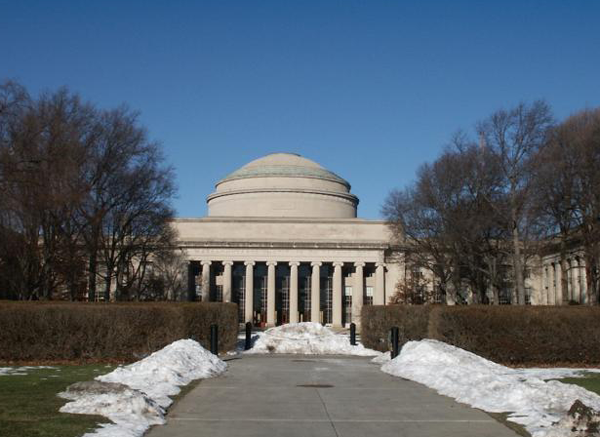
\includegraphics[width=0.9\columnwidth]{Figure1}
\caption{With Caption Below, be sure to have a good resolution image
  (see item D within the preparation instructions).}
\label{fig:figure1}
\end{figure}

\subsection{References and Citations}

Use a numbered list of references at the end of the article, ordered
alphabetically by first author, and referenced by numbers in brackets
\cite{ethics,
  Klemmer:2002:WSC:503376.503378,
  Mather:2000:MUT,
  Zellweger:2001:FAO:504216.504224}. For
papers from conference proceedings, include the title of the paper and
an abbreviated name of the conference (e.g., for Interact 2003
proceedings, use \textit{Proc. Interact 2003}). Do not include the
location of the conference or the exact date; do include the page
numbers if available. See the examples of citations at the end of this
document. Within this template file, use the \texttt{References} style
for the text of your citation.

Your references should be published materials accessible to the
public.  Internal technical reports may be cited only if they are
easily accessible (i.e., you provide the address for obtaining the
report within your citation) and may be obtained by any reader for a
nominal fee.  Proprietary information may not be cited. Private
communications should be acknowledged in the main text, not referenced
(e.g., ``[Robertson, personal communication]'').

\begin{table}
  \centering
  \begin{tabular}{|c|c|c|}
    \hline
    \tabhead{Objects} &
    \multicolumn{1}{|p{0.3\columnwidth}|}{\centering\tabhead{Caption --- pre-2002}} &
    \multicolumn{1}{|p{0.4\columnwidth}|}{\centering\tabhead{Caption --- 2003 and afterwards}} \\
    \hline
    Tables & Above & Below \\
    \hline
    Figures & Below & Below \\
    \hline
  \end{tabular}
  \caption{Table captions should be placed below the table.}
  \label{tab:table1}
\end{table}

\section{Sections}

The heading of a section should be in Helvetica 9-point bold, all in
capitals. Use Arial if Helvetica is not available. Sections should
not be numbered.

\subsection{Subsections}

Headings of subsections should be in Helvetica 9-point bold with
initial letters capitalized.  For
sub-sections and sub-subsections, a word like \emph{the} or \emph{of}
is not capitalized unless it is the first word of the heading.)

\subsubsection{Sub-subsections}

Headings for sub-subsections should be in Helvetica 9-point italic
with initial letters capitalized.  Standard {\textbackslash}section,
{\textbackslash}subsection, and {\textbackslash}subsubsection commands
will work fine.

\section{Figures/Captions}

Place figures and tables at the top or bottom of the appropriate
column or columns, on the same page as the relevant text
(see Figure~\ref{fig:figure1}). A figure or table may extend across both
columns to a maximum width of 17.78 cm (7 in.).

Captions should be Times New Roman 9-point bold.  They should be numbered (e.g.,
``Table~\ref{tab:table1}'' or ``Figure~\ref{fig:figure2}''), centered
and placed beneath the figure or table.  Please note that the words
``Figure'' and ``Table'' should be spelled out (e.g., ``Figure''
rather than ``Fig.'') wherever they occur.

Papers and notes may use color figures, which are included in the page
limit; the figures must be usable when printed in black and white in
the proceedings.  The paper may be accompanied by a short video figure
up to five minutes in length.  However, the paper should stand on its
own without the video figure, as the video may not be available to
everyone who reads the paper.

\section{Language, Style and Content}

The written and spoken language of SIGCHI is English. Spelling and
punctuation may use any dialect of English (e.g., British, Canadian,
US, etc.) provided this is done consistently. Hyphenation is
optional. To ensure suitability for an international audience, please
pay attention to the following:

\begin{itemize}
\item Write in a straightforward style.
\item Try to avoid long or complex sentence structures.
\item Briefly define or explain all technical terms that may be
  unfamiliar to readers.
\item Explain all acronyms the first time they are used in your text---e.g.,
``Digital Signal Processing (DSP)''.
\item Explain local references (e.g., not everyone knows all city
  names in a particular country).
\item Explain ``insider'' comments. Ensure that your whole audience
  understands any reference whose meaning you do not describe (e.g.,
  do not assume that everyone has used a Macintosh or a particular
  application).
\item Explain colloquial language and puns. Understanding phrases like
  ``red herring'' may require a local knowledge of English.  Humor and
  irony are difficult to translate.
\item Use unambiguous forms for culturally localized concepts, such as
  times, dates, currencies and numbers (e.g., ``1-5-97'' or ``5/1/97''
  may mean 5 January or 1 May, and ``seven o'clock'' may mean 7:00 am or
  19:00).  For currencies, indicate equivalences---e.g., ``Participants
  were paid 10,000 lire, or roughly \$5.''
\item Be careful with the use of gender-specific pronouns (he, she)
  and other gendered words (chairman, manpower, man-months). Use
  inclusive language that is gender-neutral (e.g., she or he, they,
  s/he, chair, staff, staff-hours,
  person-years). See~\cite{Schwartz:1995:GBF} for further advice and
  examples regarding gender and other personal attributes.
\item If possible, use the full (extended) alphabetic character set
  for names of persons, institutions, and places (e.g.,
  Gr{\o}nb{\ae}k, Lafreni\'ere, S\'anchez, Universit{\"a}t,
  Wei{\ss}enbach, Z{\"u}llighoven, \r{A}rhus, etc.).  These characters
  are already included in most versions of Times, Helvetica, and Arial
  fonts.
\end{itemize}

\section{Accessibility}
The Executive Council of SIGCHI has committed to making SIGCHI conferences more inclusive for researchers, practitioners, and educators with disabilities. As a part of this goal, the all authors are asked to work on improving the accessibility of their submissions. Specifically, we encourage authors to carry out the following five steps:
\begin{enumerate}
	\item Add alternative text to all figures
	\item Mark table headings
	\item Add tags to the PDF
	\item Verify the default language
	\item Set the tab order to ``Use Document Structure''
\end{enumerate}
Unfortunately good tools do not yet exist to create tagged PDF files from Latex. LaTeX users will need to carry out all of the above steps in the PDF directly using Adobe Acrobat, after the PDF has been generated.
 
For more information and links to instructions and resources, please see:
{\url{http://chi2014.acm.org/authors/guide-to-an-accessible-submission}}.

\section{Page Numbering, Headers and Footers}
Your final submission SHOULD NOT contain any footer or header string information 
at the top or bottom of each page. The submissions will be paginated in a determined 
order by the chairs and page numbers added to the pdf during the compiling, 
indexing, and pagination processes.

\section{Producing and Testing PDF Files}

We recommend that you produce a PDF version of your submission well
before the final deadline.  Your PDF file must be ACM DL
Compliant. The requirements for an ACM Compliant PDF are available at:
{\url{http://www.sheridanprinting.com/typedept/ACM-distilling-settings.htm}}.

Test your PDF file by viewing or printing it with the same software we
will use when we receive it, Adobe Acrobat Reader Version 7. This is
widely available at no cost from~\cite{acrobat}.  Note that most
reviewers will use a North American/European version of Acrobat
reader, which cannot handle documents containing non-North American or
non-European fonts (e.g. Asian fonts).  Please therefore do not use
Asian fonts, and verify this by testing with a North American/European
Acrobat reader (obtainable as above). Something as minor as including
a space or punctuation character in a two-byte font can render a file
unreadable.

\section{Blind Review}

For archival submissions, CHI requires a ``blind review.'' To prepare
your submission for blind review, remove author and institutional
identities in the title and header areas of the paper. You may also
need to remove part or all of the Acknowledgments text.  Further
suppression of identity in the body of the paper and references is
left to the authors' discretion. For more details, see the submission
guidelines and checklist for your submission category.

\section{Conclusion}

It is important that you write for the SIGCHI audience.  Please read
previous years' Proceedings to understand the writing style and
conventions that successful authors have used.  It is particularly
important that you state clearly what you have done, not merely what
you plan to do, and explain how your work is different from previously
published work, i.e., what is the unique contribution that your work
makes to the field?  Please consider what the reader will learn from
your submission, and how they will find your work useful.  If you
write with these questions in mind, your work is more likely to be
successful, both in being accepted into the Conference, and in
influencing the work of our field.

\section{Acknowledgments}

We thank CHI, PDC and CSCW volunteers, and all publications support
and staff, who wrote and provided helpful comments on previous
versions of this document.  Some of the references cited in this paper
are included for illustrative purposes only.  \textbf{Don't forget
to acknowledge funding sources as well}, so you don't wind up
having to correct it later.

% Balancing columns in a ref list is a bit of a pain because you
% either use a hack like flushend or balance, or manually insert
% a column break.  http://www.tex.ac.uk/cgi-bin/texfaq2html?label=balance
% multicols doesn't work because we're already in two-column mode,
% and flushend isn't awesome, so I choose balance.  See this
% for more info: http://cs.brown.edu/system/software/latex/doc/balance.pdf
%
% Note that in a perfect world balance wants to be in the first
% column of the last page.
%
% If balance doesn't work for you, you can remove that and
% hard-code a column break into the bbl file right before you
% submit:
%
% http://stackoverflow.com/questions/2149854/how-to-manually-equalize-columns-
% in-an-ieee-paper-if-using-bibtex
%
% Or, just remove \balance and give up on balancing the last page.
%
\balance

\section{References format}
References must be the same font size as other body text.
% REFERENCES FORMAT
% References must be the same font size as other body text.

\bibliographystyle{acm-sigchi}
\bibliography{sample}
\end{document}
